\documentclass[10pt,a4paper,notitlepage]{scrartcl}
\usepackage[utf8x]{inputenc}
\usepackage[a4paper,textwidth=17cm, top=3cm, bottom=3.5cm]{geometry}
\usepackage{eurosym}
\usepackage{url}
\usepackage[T1]{fontenc}
\usepackage{ucs}
\usepackage{ngerman}
\usepackage[ngerman]{babel} 
\usepackage{setspace}
\usepackage{times}
\usepackage{tabularx}
\usepackage{multicol}
\usepackage{hyperref}
%\usepackage[nonumberlist]{glossaries}
%\renewcommand*{\glspostdescription}{}
%\makeglossaries
\usepackage{cite}
\usepackage[pdftex]{graphicx,color}
\definecolor{p-green}{rgb}{0.12,0.57,0.11}
\usepackage{todo}
\newcommand{\gfo}{\grqq\ }
\newcommand{\gfu}{\glqq}
\newcommand{\bitem}{\item[--]}
\newcommand{\litem}[2]{\item[#1 --] #2}
\newcommand{\blitem}[3]{\item[#1 --] \texttt{#2} -- #3}
\renewcommand{\abstractname}{}
%\newcommand{\gtodo}{\textcolor{p-green}{\todos}}
%\newcommand{\sign}[1]{\begin{ttfamily}\textcolor{red}{\Large #1}\end{ttfamily}}
%\newcommand{\entwurf}{\sign{--- ENTWURF ---\\}}
\definecolor{orange}{rgb}{1,0.6,0}
\definecolor{d-green}{rgb}{0,0.8,0}
\definecolor{pink}{rgb}{1,0,0.6}
\newcommand{\annot}[1]{\textcolor{red}{#1}}
\newcommand{\sebastian}[1]{\textcolor{pink}{#1}}
\newcommand{\konrad}[1]{\textcolor{blue}{#1}}
\newcommand{\jens}[1]{\textcolor{orange}{#1}}
\newcommand{\robert}[1]{\textcolor{d-green}{#1}}
\newcommand{\ecolor}[1]{\textcolor{pink}{#1}}
\onehalfspacing
\setlength{\parskip}{6pt plus4pt minus4pt}

%\usepackage{draftcopy}
%\usepackage[printwatermark=true,allpages=true,fontfamily=pag,
%	color=gray!25,textmark=I am happy,angle=45,fontsize=5cm,
%	width=\paperwidth,fontseries=b,scale=0.8,
%	xcoord=0,ycoord=0]{xwatermark}
\usepackage{draftwatermark}

\begin{document}
\begin{center}
\vspace*{-1cm}
\textsf{\Huge Heutige Anforderungen an den\\
Internetzugang in der Schule}\\
\bigskip
\large Zusammengestellt von internetaffinen\\
SchülerInnen der Landesschule Pforta\\
\vspace*{1cm}
\begin{tabularx}{\textwidth}{XXX}
	\begin{minipage}{5cm}
		\begin{center}
			\small Jan Sebastian Götte\\
			\small \texttt{<s@twopi.de>}
		\end{center}
	\end{minipage}&
	\begin{minipage}{5cm}
		\begin{center}
			\small Jens Oliver John\\
			\small \texttt{<joj@twopi.eu>}
		\end{center}
	\end{minipage}&
	\begin{minipage}{5cm}
		\begin{center}
			\small Robert Hemstedt\\
			\small \texttt{<robs@twopi.eu>}
		\end{center}	
	\end{minipage}
\end{tabularx}
\end{center}
\bigskip
%Notwendigkeit!!!
\setlength{\columnsep}{-1cm}
\begin{multicols}{2}
\begin{abstract}
In einer Institution mit Tradition, in einem Internatsgymnasium mit dem Anspruch, sich in den oberen Teil der Liste der Ausbildungsstätten der zukünftigen Eliten Deutschlands einzureihen, obliegt es der Verantwortung der Schüler jener Schulen, ihre Lehrkräfte in ihrem Bestreben, den Schülern jene Mittel an die Hand zu geben, die zum Erreichen des angestrebten Modus docendi als zeitgemäß oder vonnöten angesehen werden, nach bestem Wissen und in eigener Initiative durch Äußerungen des Schülerwillens zu unterstützen und ihnen bezüglich der Planung nach bestem Vermögen und Gewissen Informationen zukommen zu lassen.
\end{abstract}
\end{multicols}
\tableofcontents
\newpage % This is just a reminder. I think the first page will be pretty crammed. If it spans two pages, consider moving the whole toc to the second page.

\setlength{\columnsep}{1cm}
\section{Zeitgemäße Internetanbindung: Das Was und Warum}
\subsection{Über die Notwendigkeit in sozialer und pädagogischer Hinsicht}
\begin{multicols}{2}
Es gibt das Internet inzwischen seit 20 Jahren. Seit seinem Beginn als Netzwerk von Forschungscomputern avancierte es zu einem allgegenwärtigen Medium der Information, Kommunikation und Bildung. Kein Schüler kommt umher, ohne das Internet zu nutzen, sei es um Kontakte zu pflegen, um sich für einen Vortrag vorzubereiten oder um sein Dussmann-Schulessen zu bestellen. Die Stoffpläne für den Unterricht werden durch das Kultusministerium Sachsen-Anhalts online zur Verfügung gestellt, die Wikipedia stellt vielen Schülern eine wichtige Grundlage für Kurzvorträge und Referate und E-Mail, ICQ, IRC und Jabber ermöglichen N-ies den Kontakt mit Praktikumsbetreuern und allen den Kontakt mit geographisch entfernten Freunden.

Es ist Aufgabe der Schule, uns die allgemeine Hochschulreife zu vermitteln. Das bedeutet heute auch den sicheren Umgang mit Medien wie dem Internet. Ein Schüler, der nach seinem Abitur noch immer nicht im Internet recherchieren kann und sich nicht vor den Gefahren des Internets -- Viren, Botnets, Trojaner, Phishing, Sniffing, Spam, Scam etc.\ -- zu schützen vermag, hat seinen Kommilitonen gegenüber einen erheblichen Nachteil. Auch fast jeder Beruf mit Ausnahme einiger weniger Handwerke wie dem des Bauarbeiters erfordert den sicheren Umgang mit dem Computer. Ein Schüler der die vier Jahre vor seinem Abitur zuhause selbstverständlich den Computer und das Internet nutzte ist hier einem Schüler, der jeden Tag -- das Wochenende eingeschlossen -- zur Nutzung seiner zweistündigen Internetzugangsmöglichkeit in seiner Freizeit durch die Schule laufen musste überlegen. Schüler von heute müssen so früh wie nur möglich an die Technologien von heute herangeführt werden und dürfen nicht bis zu ihrem Studium von diesen fern gehalten werden, um mit dem Studienbeginn den Gefahren und Chancen unvorbereitet ausgesetzt zu sein.

Zuletzt ist das Internet auch ein wichtiges wenn nicht das wichtigste Medium für aktuelle Nachrichten. Es bietet eine Fülle von fachspezifischen Nachrichtenseiten, mit deren Angebot das Studienzentrum auch nicht entfernt zu konkurrieren vermag.
\end{multicols}
%Notwendig weil allgegenwärtig ==> Entwicklung von Softskills nötig
%	Medienkompetenz
%		Gefahren kennen
%			Viren
%			Botnets
%			Spam
%			Phishing
%			Sniffing
%			Scam
%Nachrichten/Information: schulisch wie außerschulisch; enorme Fülle
%	DIE Quelle
%Leben in Pforte - Freizeitgestaltung
%Kommunikation/Soziale Kontakte
%	nach hause - heimfahrten?
%		beispielsweise bahn.de, google maps, openstreetmap
%	in andere länder
\subsection{Technische Anforderungen}
\begin{multicols}{2}
Moderne Nutzung des Internets erfordert eine hohe Bandbreite und eine geringe Latenz. Bandbreite ist für das Ansehen von Videos wichtig\footnote{z.B.\ die Vorlesungsaufzeichnungen verschiedener Projekte wie des OpenCourseWare Project des MIT}	-- ein Richtwert für  das Minimum kann hier 2MBit/s sein, was 250 kByte/s entspricht. Eine geringe Latenz ist für Anwendungen wie Chatrooms\footnote{ein weit verbreitetes Protokoll ist IRC, IRC-Channel werden häufig von Softwareentwicklern zur Koordination verwendet.} und VoIP (z.B.\ Skype) wichtig. Eine hohe Zuverlässigkeit der Internetverbindung ist ebenfalls notwendig, da sonst große Downloads\footnote{Die Installations-DVD eines Linux-Betriebssystems ist ohne weiteres 4GB groß} nicht fertig gestellt werden können. Bezüglich der Zuverlässigkeit einer Internetverbindung sind 99\% nicht viel -- das restliche Prozent entspricht knapp einer Viertelstunde Ausfallzeit pro Tag.

Des weiteren muss ein schülerfreundlicher Internetzugang, der den Anforderungen an den Bildungsauftrag der Schule entspricht, unbedingt unzensiert sein. Der Einsatz von Filtersoftware zieht immer \gfu Kollateralschaden\gfo mit sich. Die Sperrung normaler Webseiten ist nicht verhinderbar.
Filterlisten müssen gewartet werden. Diese Wartung kostet Zeit und damit Geld --- der Aufwand ist so groß, dass es für eine Schule wie Schulpforte unmöglich ist, diesen Aufwand zu bewerkstelligen. Eine Filterung der Internetzugriffe auf Basis einer Whitelist ist unpraktikabel, da es um einige Zehnerpotenzen zu viele Webseiten gibt um auch nur einen mikroskopischen Bruchteil zu indizieren.

Wir möchten darauf hinweisen, dass der Großteil dessen, was man im Internet finden kann, völlig normale Webseiten sind. Illegale oder Jugendgefährdende Angebote bilden nur einen extrem geringen Anteil und jemand, der es darauf anlegt kann jede Sperre mit geringem Aufwand umgehen. Eine Aufzeichung der Internetzugriffe durch Schüler ist wie eine Filterung äußerst aufwändig und kostenintensiv und produziert eine Datenmenge, die für eine Auswertung bei weitem zu groß ist. Im Zweifelsfall sind solche geloggten Daten nicht belastbar, da sowohl MAC-Adresse als auch IP-Adresse und Computername sehr einfach fälschbar sind und mehrere einfache Techniken zur Umgehung dieser Logs existieren. Letztlich sind die benannten Logs auch datenschutzrechtlich und bezüglich des Briefgeheimnisses bedenklich.

Um von großem Nutzen zu sein muss der Internetzugang überall verfügbar sein. Eine Lösung wie momentan, bei der wir ständig zwischen Studienzentrum (\gfu Internet\grqq) und Zimmer pendeln müssen, ist zur ernsthaften Arbeit unpraktikabel. Zur effektiven Recherche und Unterrichtsvorbereitung ist es notwendig, das man von seinem Schreibtisch, wo man auch alle Unterlagen hat und alle Schulbücher sind, auf das Internet zugreifen kann. Auch technisch ist es nicht besonders sinnvoll, zu versuchen, die Internetzugangsmöglichkeiten auf bestimmte Orte zu beschränken, da die elektromagnetischen Wellen eines WLANs -- wie jeder Physiklehrer bestätigen wird -- nicht an den Wänden eines Raumes \gfu anhalten\grqq, sondern selbst aus 50 Meter Entfernung noch empfangbar sind.

Damit große Downloads\footnote{Auch hier sei auf die mehrere Gigabyte großen Installationsdateien des Linux-Betriebssystems verwiesen} bevorzugt nachts laufen, um die Leitung nicht zu verstopfen und den restlichen Verkehr nicht zu behindern sollte es die Möglichkeit geben, diese nachts durchzuführen. Wir möchten darauf hinweisen, dass Schüler, die es darauf anlegen auch bei einer Abschaltung des Internetzugangs ins Netz kommen. Im Rahmen der durch unser Schulprogramm propagierten Eigenverantwortlichkeit, die man von einem intelligenten Schüler der Landesschule Pforta erwarten sowie durch die DHL kontrollieren kann, ist davon auszugehen, dass niemand nachts das Internet benutzt. Hier funktionieren dieselben Selbstkontrollmechanismen die schon bei übermäßigem Konsum von Computerspielen funktionieren.

\hyphenation{Black-VPN}
Um die Schüler vor Internetkriminalität sowie dem bezüglich Datenschutz problematischen Tracking und Angriffen durch Cracker zu schützen, ist die Verwendung eines VPN-Dienstes wie IPREDator, SwissVPN, BlackVPN etc.\ wünschenswert. Ein günstiger Nebeneffekt solcher Maßnahmen wäre, dass eine versehentliche Urheberrechtsverletzung durch einen Schüler so nicht auf die Schule zurückzuführen wäre.
\end{multicols}




%schnell: >2Mbit/schüler
%zuverlässig: 99% verfügbarkeit sind _nicht_ viel
%frei%
%		ungefiltert: wer mist will kommt auch an mist ran
%		ungeloggt: alle logs lassen sich umgehen und sogar fälschen
%			zufälliger log-poison ist legal und verhindert missverständnisse
%	filter sowie logs brauchen wartung - hohe kosten, bei derzeitiger lage völlig utopisch
%überall
%	warum irgendwo nicht? internet ist per definition nicht beschränkbar => bitte physiklehrer nach ausbreitungscharakteristika von 2.4GHz-Wellen fragen.
%rund um die uhr
%	selbstverantwortlichkeit - siehe schulkonzept
%		wer mist bauen will kann auch hier mist bauen
%	massive downloads (freie linux-distro-dvds etc.) belasten die bandbreite und sollten nachts laufen
%	internationalität: um 5 ist es in amerika 8 abends
%anonymisiert (VPN etc.) für mehr Datensicherheit, gegen geolocation etc.
%	nebeneffekt: abmahnungen erreichen die schule nicht
%
\section{Status pfortensischer Internetanbindung}
\subsection{Fakten}
\begin{multicols}{2}
Derzeit gibt für Schüler Pfortes die folgenden Internetzugangsmöglichkeiten:
\begin{enumerate}
  \item Das Studienzentrum
\end{enumerate}
Das Studienzentrum hat von Montag bis Donnerstag, jeweils während der Schulzeit, einschließlich eines großen Teiles der Mittagspause, von 7.30 bis 16.00 Uhr geöffnet sowie über dieselben Tage von 19.00 bis 21.00 Uhr im Abendbereich. Zudem besteht für Schüler der elften und zwölften Klassen die Möglichkeit der Nutzung des Studienzentrums während des Silentiums, für Elftklässler nurmehr unter Aufopferung einer Portion \gfu Sile-Frei\grqq. Das Studienzentrum ist per DSL bei für fast alle Anwendungszwecke akzeptablen Latenzen mit einer Geschwindigkeit von 2MBit/s an das Internet angeschlossen. Die Mehrheit der Schüler nutzt das Studienzentrum aufgrund von Unterricht und Silentium während der abendlichen Öffnungszeiten (sofern dann keine Arbeitsgemeinschaften statt finden und Schüler des musischen Zweiges nicht durch den Chor gebunden sind), was in durchschnittlich ca. 20 anwesende Schüler mit Notebooks sowie 12 besetzte Schulcomputer mündet. Die jedem Schüler in diesem Fall (davon ausgehend, dass niemand versucht, eine große Datei wie eine Aufzeichnung der aktuellen Tagesschau herunterzuladen) theoretisch zur Verfügung stehende Bandbreite liegt bei ca. 7 kByte/s, das entspricht der Geschwindigkeit eines analogen Modems.
\end{multicols}
%stuze: 2mbit
%sonst exakt nichts
%viel zu wenig, völlig überlastet ==> berechnen
%zu wenig zeit
%
\subsection{Mißstände}
\begin{multicols}{2}
Es ist sowohl die Liste der Internetzugangsmöglichkeiten mit exakt einer erheblich zu kurz als auch deren Bandbreite und Zuverlässigkeit viel zu gering. Die Geschwindigkeit die das Studienzentrum bietet galt schon vor einem Jahrzehnt als veraltet - heute reicht sie kaum um einfache Webseiten wie Blogs zu betrachten.

Heute spielt sich auch ein Teil des Soziallebens junger Menschen immer weiter im Internet in sozialen Netzwerken wie dem \emph{MyTalent}-Portal von Fraunhofer ab. Die schlechen Zugangsmöglichkeiten zum Internet nehmen den Schülern die Möglichkeit diesen Teil ihres Soziallebens adäquat zu pflegen und wie inzwischen möglich Kontakt mit anderen Schülern aus aller Welt zu halten.

Ein weiterer Mangel ist, dass alle Schüler gezwungen sind, sich entweder ein teures Notebook zu kaufen oder die vollkommen veralteten Schulcomputer zu benutzen, da es bei der momentanen Ausführung für Schüler unmöglich ist, einen eigenen Standcomputer zu verwenden.
\end{multicols}
%unzuverlässig (instabil)
%schüler mit eigenen festen computern können diese nicht benutzen
%soz. netzwerke wie mytalent-portal von fraunhofer sowie der kurznachrichtendienst twitter nicht nutzbar weil zu lahm und zu wenig zeit und zu weite wege
%nachwuchs wird abgeschreckt
%
%Auftrag der Schule: allg. Hochschulreife
%	Schüler müssen lernen, mit Technik umzugehen
%	lernen zu recherchieren
%
\section{Lösungsansätze, -vorschläge}
\subsection{Bei minimalen Kosten}
\begin{multicols}{2}
Um die Kosten gering zu halten, gilt es zwei Grundsätze zu beachten:
\begin{enumerate}
\item Teure Spezialhard- und -software vermeiden
\item Bestehende Infrastrukturen möglichst weitgehend verwenden
\end{enumerate}
Ersterer vermeidet das so genannte \gfu Vendor Lock-In\grqq, den Zustand, bei dem weitere Investitionen durch bestehende Systeme an einen Hersteller gebunden sind. Letzterer vermeidet das besonders in Altbauten kostenaufwändige Verlegen neuer Kabel.

In Pforte sind die bestehenden Infrastrukturen die Telefonleitungen, durch die sich innerhalb Pfortes geschätzt 10Mbit/s pro Leitung transportieren lassen sowie die Fernsehkabel, die theoretisch Bandbreiten im Bereich von 100Mbit/s ermöglichen. Die Internetanbindung Pfortes kann durch eine Kombination aller verfügbaren Technologien (DSL und TV-Kabel) erreicht werden. Die hierbei notwendige Leitungsbündelung kann durch einen günstigen Server oder durch eine teurere spezialisierte Lösung geschehen. Alternativ kann auch auf jedem Flur ein Router mit eigenem DSL-Anschluss aufgestellt werden, was aber höhere Betriebskosten mit sich zieht und relativ unflexibel ist.

Nachteil einer solchen Lösung ist, dass die verwendeten Technologien definitiv nicht \gfu state-of-the-art\gfo sind und in einigen Jahren einer teuren Erneuerung bedürfen.
\end{multicols}
%bestehende infrastruktur nutzen: fernsehkabel/dsl
%durch router pro flur (dsl) näherungsweise brauchbare geschwindigkeiten herzaubern
%kontra: technisch völlig veraltet - nicht zeitgemäß
\subsection{Bei möglichst gutem Kosten/Nutzen-Verhältnis}
\begin{multicols}{2}
Bestehende Infrastrukturen sind im Falle der Netzanbindung Pfortes die praktikabelste Lösung, da neue Kabel sehr hohe Kosten mit sich ziehen. Die Bündelung mehrerer Leitungen kann durchaus für zeitgemäße Geschwindigkeiten sorgen. Innerhalb von Schulpforte würde man die Weiterverteilung mit Glasfaserkabeln (nicht so teuer wie es sich anhört) zwischen den Internaten und innerhalb der Internate mit normalen Netzwerkkabeln (mind.\ Cat 6) lösen. Pro Flur gäbe es WLAN-Zugangspunkte (APs) und optimalerweise Ethernet-Anschlüsse auf den Zimmern. Eine solche Lösung würde es ermöglichen, ohne Veränderung der teilweise neuen Infrastruktur in Schulpforte den Anschluss Schulpfortes später auf Glasfaserverbindungen umzustellen, da die Bandbreite von Netzwerkkabeln sowie Glasfaserleitungen auf absehbare Zeit für alle Anwendungsgebiete ausreicht.
\end{multicols}
%durch bestehende infrastrukturen (fernsehkabel/dsl/richtfunk) nach pforte, dann durch bei bedarf nachgerüstete netze in die internate und internatsintern auf die flure und von dort per wlan weiter
%\subsection{Auf neuer Infrastrukut basierend}
%glasfaser nach pforte für optimale geschwindigkeit und zukunftsfestigkeit
%innerhalb pfortes über glasfaser in die internate
%im internat sowohl per copper-lan als auch per wlan verteilt
\subsection{Unter Verwendung neuer Infrastruktur}
%Glasfasern nach Pforte
%Glasfasern in die Internate
%LAN und WLAN auf den Zimmern
\begin{multicols}{2}
Letztendlich wäre es wünschenswert wenn auch die Netzanbindung Pfortes durch Glasfaserkabel geschieht, welche auf absehbare Zeit genügend Bandbreite bieten werden. LAN-Anschlüsse auf den Zimmern sind angesichts der beschränkten Bandbreite von WLAN und der großen Nähe der Schülercomputer notwendig -- auch um Schüler ohne (teure) WLAN-Karte Internetzugang zu bieten.

Zu beachten ist, dass Lösungsvorschlag 2 nachträglich relativ problemlos zu Lösungsvorschlag 3 aufgerüstet werden kann, Lösungsvorschlag 1 den anderen beiden gegenüber jedoch weitgehend inkompatibel ist.
\end{multicols}
\section{Schlusswort}
\begin{multicols}{2}
Wir wünschen uns, dass die bisher in Pforte von offizieller Seite vorherrschende Einstellung des \gfu Innovationsprotektionismus\gfo beendet wird und moderne Technologien, so selbstverständlich wie diese in der restlichen Gesellschaft sind, umgesetzt werden. Um nach 500 Jahren noch immer konkurrenzfähig zu bleiben und weiterhin ein magnetischer Monopol für die Elite von morgen zu sein, muss sich Pforte den Gegebenheiten der heutigen Welt anpassen und Veränderungen wie das Aufkommen des Internets nicht noch nach 20 Jahren leugnen und verachten.

Bezüglich der technischen Kontrolle und Überwachung der Internetanbindung der Schüler weisen wir darauf hin, dass jede Art dieser selbst durch wenig begabte Schüler umgehbar ist. Die Mechanismen, die den Missbrauch moderner Technologien in Pforte bisher verhinderten, Kontrollen durch im \gfu Real-Life\gfo in die Zimmer kommende Lehrer und durch den ausgleichenden Effekt des engen sozialen Geflechts in Pforte, werden diesen Missbrauch auch bei einer besseren Verfügbarkeit besagter Technologien weiterhin verhindern. Eine Zimmerkameradin ist effektiver als jede Logdatei, da die Logdatei erst noch angeschaut werden muss, was bei einem Aufkommen von 300 Stück täglich unmöglich sein dürfte. Das Potential, verbotene Dinge zu tun wird durch die Ausweitung der Verfügbarkeit der Internetzugangsmöglichkeiten in Schulpforte nicht größer. Schüler, die die Regeln unserer Gemeinschaft missachten, haben offenbar einige Grundgedanken Pfortes nicht verstanden und werden sich durch nichts als gute Argumente, Mitschüler und die natürliche Entwicklung aufhalten lassen.

\sebastian{Zu radikal?}
Eine letzte Anmerkung zu Kontrolltechnologien sei noch angebracht: All diese Techniken haben auch eine politische Dimension. Sie widersprechen der Philosophie des Internets --- das Internet wurde designt um exakt diese Techniken möglichst stark zu erschweren --- und wurden ursprünglich von Staaten wie China, Saudi-Arabien und Iran entwickelt, die mit ihnen die Meinung ihrer BürgerInnen kontrollieren und unterdrücken wollen. Wir möchten keinesfalls die Gründe, die in Pforte für den Einsatz solcher Technologien sprechen, auf eine Stufe mit der Zensur der genannten undemokratischen Regime stellen, möchten jedoch anmerken, dass wir es durchaus bedenklich finden, dass solche Techniken an unserer Schule zur Kontrolle der Schüler Anwendung finden sollen.
\end{multicols}
%schluss mit dem "innovationsprotektionismus"
%
%=== wer mist bauen will kann auch jetzt schon mist bauen! denselben mist! ===
%Chaospotential wird _nicht_ größer
%"illegale" downloads sind üblich, 80%*belegen der Internetnutzer machen diese!!
%
%zum schluss ein politisches argument gegen filterinfrastrukturen:
%	wir wollen uns nicht auf eine stufe mit ländern wie china, saudi-arabien, iran stellen.
%

\newpage\appendix
\section*{\huge Anhang}
\section{Kurzzusammenfassung}
Für einen schülerfreundlichen Internetzugang in Schulpforte sind die folgenden Punkte wünschenswert:
\begin{enumerate}
\item Internet \textbf{auf den Zimmern} (optimalerweise auch auf großen Teilen des Schulgeländes, z.B. in den Unterrichtsräumen)
\item Internet \textbf{ohne Zeitbeschränkung} (Im Sile zur Recherche und für den Download großer Dateien außerhalb der Hauptnutzungszeiten)
\item \textbf{Neutrales} Internet, das heißt Internet ohne Filtermaßnahmen
\item \textbf{Anonymes} Internet, das heißt Internet ohne schülerbezogene Mitschnitte
\item \textbf{Schnelles} Internet (mindestens 2 Mbit/s pro Schüler)
\end{enumerate}

\section{Links und weiterführende Informationen}
\vspace{-1.5cm}
\nocite{*}
\bibliographystyle{plain}
\renewcommand{\refname}{}
\bibliography{links}
\bigskip

\section{Begriffe}
\begin{description}
\blitem{AP}{Access Point}{WLAN-Zugangspunkt}
\litem{Bandbreite}{Gleichzeitig übertragbare Datenmenge}
\litem{BitTorrent}{Protokoll zur Veröffentlichung großer Dateien}
\litem{Ethernet}{Drahtgebundenes LAN}
\litem{Fiber Optics}{Glasfaser}
\litem{Freifunk}{WLAN-System, bei dem die Daten jeweils über die kürzeste Kette von Access Points weitergeleitet werden}
\blitem{FTP}{File Transfer Protocol}{Heute nur noch selten verwendetes Protokoll zum Herunterladen von Dateien}
\litem{Hierarchisches Netzwerk}{Netzwerk, bei dem die Computer und Switches bzw.\ Router in einer Baumstruktur angeordnet sind}
\blitem{HTTP}{Hyper Text Transfer Protocol}{Datenformat zum Abrufen von Internetseiten}
\blitem{IP-Adresse}{Internet Protocol-Adresse}{(Veränderliche) Netzwerkadresse eines Computers}
\blitem{IRC}{Internet Relay Chat}{System zum Versenden von Kurznachrichten und Dateien zwischen mehreren Personen}
\litem{IRC-Channel}{Chatroom auf einem IRC-Server}
\blitem{LAN}{Local Area Network}{Computernetzwerk}
\litem{Latenz}{Zeit, die ein Datenpaket vom Startcomputer zum Zielcomputer benötigt}
\litem{Logging}{Aufzeichnung von Daten zur späteren Auswertung}
\blitem{MAC-Adresse}{Media Access Control Adresse}{Computerspezische Netzwerkadresse}
\litem{Mesh-Netzwerk}{Vermaschtes (nicht-hierarchisches) Netzwerk, bei dem die Daten jeweils den kürzesten Weg nehmen}
\blitem{NAT}{Network Address Translation}{Verwendung einer IP-Adresse für mehrere Computer}
\blitem{NIC}{Network Interface Card}{Netzwerkkarte}
\litem{Ping}{Synonym für \emph{Latenz}}
\blitem{PoE}{Power over Ethernet}{Stromversorgung über Netzwerkkabel}
\litem{Protokoll}{Datenübertragungsformat}
\litem{Router}{\gfu LAN-Verteiler\gfo mit der Fähigkeit, intelligent über die Übermittlungswege zu entscheiden}
\litem{Server}{Computer, der Internetdienste wie Webseiten oder E-Mail anbietet}
\litem{State of the art}{Auf dem aktuellen Stand der Technik}
\litem{Switch}{\gfu LAN-Verteilerdose\gfo}
\litem{Tracking}{Unwissentliche Verfolgung eines Benutzers durch einen Werbedienstleister über mehrere Webseiten zur Erstellung eines Nutzungsprofils}
\blitem{VoIP}{Voice over Internet Protocol}{Internettelefonie}
\blitem{VPN}{Virtual Private Network}{Eine Technik, die eingesetzt wird, um den gesamten Datenverkehr eines Internetnutzers verschlüsselt zu übertragen und zur Anonymisierung mit dem weiterer Internetnutzer zu mischen}
\blitem{WAN}{Wide Area Network}{Computernetzwerk über große Entfernungen (z.B.\ DSL)}
\blitem{WDS}{Wireless Distribution System}{Zusammenschluss mehrerer WLANs}
\litem{Whitelist}{Eine Liste erlauber Begriffe bzw.\ Webseiten}
\blitem{WLAN}{Wireless LAN}{Drahtloses Computernetzwerk}
\end{description}
%\printglossaries

\newpage
\section{Umrechnungstabellen}
\begin{center}
\begin{tabularx}{8cm}{r|l|l}
\textbf{SI-Vorsatz}&\textbf{Byte}&\textbf{Bit}\\
\hline
&$1$&$8$\\
Kilo-&$1.000$&$8.000$\\
Mega-&$1.000.000$&$8.000.000$\\
Giga-&$1.000.000.000$&$8.000.000.000$\\
Tera-&$1\cdot 10^{12}$&$8\cdot 10^{12}$\\
Peta-&$1\cdot 10^{15}$&$8\cdot 10^{15}$\\
Exa-&$1\cdot 10^{18}$&$8\cdot 10^{18}$
\end{tabularx}
\hspace{5mm}
\begin{tabularx}{8cm}{r|l|l}
\textbf{SI-Vorsatz}&\textbf{Bit}&\textbf{Byte}\\
\hline
&$1$&$0.125$\\
Kilo-&$1.000$&$125$\\
Mega-&$1.000.000$&$125.000$\\
Giga-&$1.000.000.000$&$125.000.000$\\
Tera-&$1\cdot 10^{12}$&$125\cdot 10^{9}$\\
Peta-&$1\cdot 10^{15}$&$125\cdot 10^{12}$\\
Exa-&$1\cdot 10^{18}$&$125\cdot 10^{15}$
\end{tabularx}
\end{center}
\begin{center}
\begin{tabularx}{8cm}{r|l}
\textbf{Bit}&\textbf{Byte}\\
\hline
1 kBit&125 Byte\\
2 kBit&250 Byte\\
1 MBit = 1.000 kBit&125 kByte\\
2 MBit = 2.000 kBit&250 kByte\\
1 GBit&125 MByte\\
\end{tabularx}
\hspace{5mm}
\begin{minipage}{8cm}
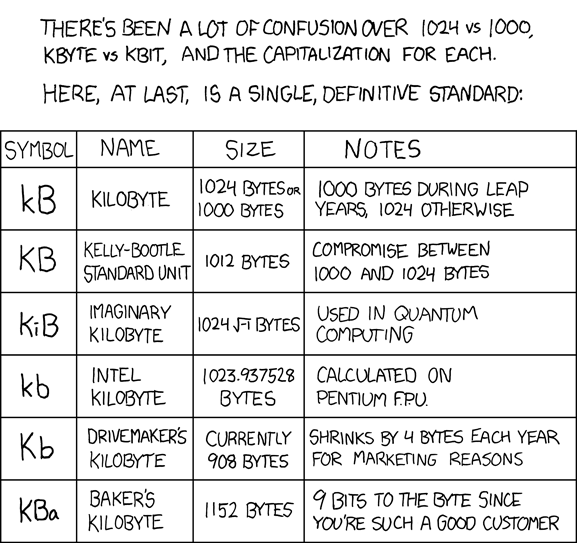
\includegraphics[width=8cm]{0394-kilobyte.png}
\end{minipage}
\end{center}
\vspace{2mm}
\begin{center}
\begin{tabularx}{8cm}{r|l}
\textbf{Basis 1024}&\textbf{Basis 1000}\\
\hline
1 kB&1000 B\\
1 MB&976,6 kiB\\
1 GB&953,674.3 MiByte\\
1 TB&931,322.574.6 GiB
\end{tabularx}
\hspace{5mm}
\begin{tabularx}{8cm}{r|l}
\textbf{Basis 1000}&\textbf{Basis 1024}\\
\hline
1 kiB&1024 B\\
1 MiB&1.048,576 kB\\
1 GiB&1.073,741.824 MByte\\
1 TiB&1.099,511.628 GB
\end{tabularx}
\end{center}
\newpage

\section{Möglichkeiten des Loggings und der Filterung}
\begin{multicols}{2}
Prinzipiell sind zwei Arten der Speicherung von durch Schüler verursachte Daten möglich: Die Speicherung von Verbindungsdaten erlaubt es, im Nachhinein Zeitpunkt, Quell-MAC- und Quell-IP-Adresse sowie den Ziel-Host zu bestimmen. Am Beispiel der URL \url{http://www.getdigital.de/products/Life_is_too_short_for_56k} ist der Zielhost \url{www.getdigital.de}. Auf DNS-Ebene lassen sich auch einzelne Domainnamen sperren (\nolinkurl{spiegel.de}, \nolinkurl{.cn}, \nolinkurl{ftp.ccc.de}).

Die zweite Möglichkeit wird Deep Packet Inspection (DPI) genannt und umfasst auch eine Durchsuchung des gesamten Datenpaketinhaltes. Dabei werden neben der vollständigen URL auch die Inhalte der aufgerufenen Web-Seiten gespeichert sowie sog. Session-Cookies durchsucht.

Zu Methode 1: Eine Speicherung von verbindungsbezogenen Daten (Vorratsdatenspeicherung) erachten wir als unverhältnismäßigen Eingriff in die Privatspäre der Schüler. Vor kurzem erst wurde die von der Bundesregierung ausgearbeitete Variante einer solchen Speicherung durch das Bundesverfassungsgericht als unverhältnismäßig abgelehnt. Ein weiterer Nachteil solcher Technik ist der hohe Wartungs- und Konfigurationsaufwand. Eine (v.a.\ gegen unberechtigten Zugriff) sichere Speicherung dieser Daten ist für eine relativ kleine Institution wie unsere Schule ohne nennenswerte IT-Kapazitäten schwer realisierbar.

Zu Methode 2: Deep Packet Inspection ist zugleich ein sehr tiefer Eingriff in die Privatsphäre der Schüler, da mit ihr jede E-Mail, jede Facebook-Profilseite durchsucht und gefiltert wird. Sollten hier gespeicherte Daten gehackt werden, wäre der Schaden groß.

Eines der Hauptprobleme von DPI ist, dass die Kosten (Anschaffung, Strom, Wartung) sehr hoch sind und eine gute Wartung der Filtersysteme Voraussetzung ist, da ein Ausfall des Filtersystems die Internetanbindung der gesamten Schule kappen würde. Bei der avisierten Bandbreite sind solche Filtersysteme enorm aufwändig und in Anschaffung wie Betrieb entsprechend teuer.

Ein Kritikpunkt aller Systeme ist die leichte Umgehbarkeit. Die erstgenannten Techniken (sowohl Filter als auch Sperrung) sind bei Schülern mit einem gewissen Maß an Medienkompetenz, wie es in Pforte weit verbreitet ist, und die der Bedienung von Google kundig sind, nicht sehr hilfreich, da sie sehr einfach umgangen werden können (siehe: Diskussion zum \glqq Zugangserschwerungsgesetz\grqq, es existieren YouTube-Videos, die das Umgehen von DNS-Sperren in weniger als einer Minute erklären).
DPI-Systeme sind schwerer zu umgehen, jedoch können die Sperren z.B.\ mittels eines sog.\ Webproxys auch von Schülern einfach umgangen werden. Die Sperrung von Webproxys ist technisch unmöglich, da sie in zu großer Anzahl vorhanden sind. Die Erhebung von Verbindungsdaten via DPI kann vom Schüler durch die Verwendung sicherer Protokolle wie HTTPS, SSH oder VPN umgangen werden.
\end{multicols}
\newpage
\section*{Changelog des Dokumentes}
\begin{tabularx}{\textwidth}{r|l}
\textbf{Version}&\textbf{Anmerkungen}\\\hline
0.1&Ursprüngliche Version, zur Veröffentlichung am 27.08. eingereicht
\end{tabularx}
\end{document}